\section{CHƯƠNG 9: MỘT VÀI CÔNG CỤ BỔ TRỢ CHO VIỆC PHÁT TRIỂN KÊNH TIKTOK} \label{sec:aux_tool}

\subsection{Giới thiệu chung}

Bên cạnh công cụ cốt lõi là \textbf{công cụ hỗ trợ viết kịch bản cho video TikTok} dựa trên phân tích dữ liệu (đã trình bày ở các chương trước), nhóm nhận thấy nhu cầu của các nhà sáng tạo nội dung còn mở rộng ra các giai đoạn khác trong quá trình sản xuất video. Để đáp ứng nhu cầu này và cung cấp một bộ giải pháp toàn diện hơn, nhóm đã phát triển thêm hai công cụ bổ trợ: \textbf{công cụ hỗ trợ nghiên cứu chủ đề} và \textbf{công cụ gợi ý cách quay video ẩm thực}.

\subsection{Công cụ hỗ trợ nghiên cứu chủ đề}

% Insert image
\begin{figure}[H]
    \centering
    % Insert border box
    \frame{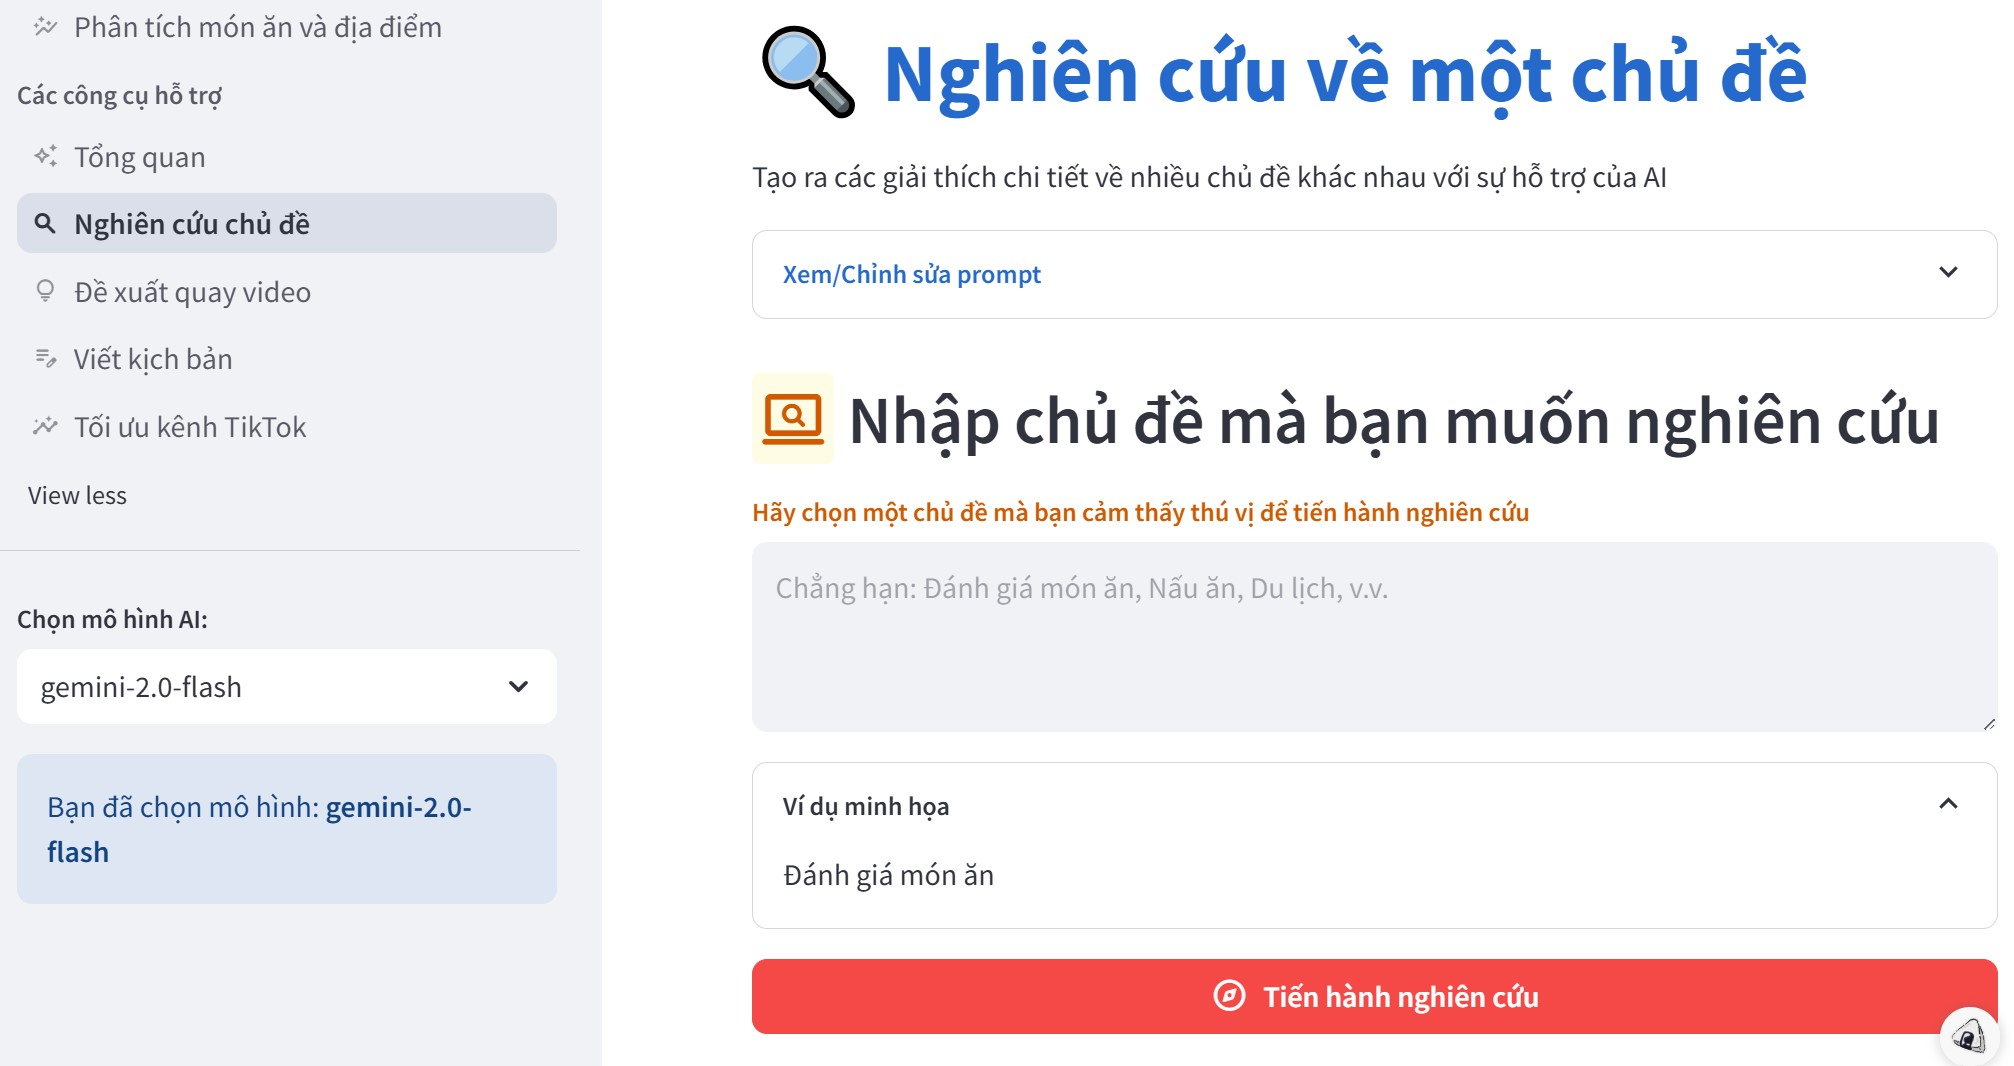
\includegraphics[width=0.99\linewidth]{img/21127739/research/research_main_page.jpg}}
    \caption{Giao diện chính của công cụ hỗ trợ nghiên cứu chủ đề}
    \label{fig:research_main_page}
\end{figure}

\subsubsection{Tổng quan}

Trong quá trình phát triển kênh TikTok, việc khám phá và thử nghiệm các chủ đề nội dung mới là yếu tố quan trọng để thu hút và giữ chân khán giả. Tuy nhiên, đối với những chủ đề mà nhà sáng tạo nội dung chưa có nhiều kinh nghiệm hoặc kiến thức nền tảng, giai đoạn nghiên cứu ban đầu có thể tốn nhiều thời gian và công sức. Để giải quyết vấn đề này, bên cạnh công cụ hỗ trợ viết kịch bản dựa trên phân tích dữ liệu TikTok, nhóm đã phát triển một công cụ bổ trợ độc lập: \textbf{Công cụ Hỗ trợ Nghiên cứu Chủ đề}.

Công cụ này được thiết kế như một \textbf{trợ lý nghiên cứu ảo}, giúp người dùng nhanh chóng tổng hợp và cấu trúc thông tin về một chủ đề bất kỳ mà họ quan tâm. Điểm khác biệt chính so với công cụ hỗ trợ viết kịch bản là công cụ này \textbf{không dựa trên việc phân tích các đặc trưng dữ liệu đã được rút trích từ video TikTok}, mà thay vào đó, nó khai thác sức mạnh của các Mô hình Ngôn ngữ Lớn (Large Language Models - LLMs) thông qua \href{https://ai.google.dev/}{Gemini API} của Google. Phần này sẽ trình bày chi tiết về mục tiêu, kiến trúc, các kỹ thuật chính được sử dụng và quy trình hoạt động của công cụ này.

\subsubsection{Mục tiêu và Lợi ích}

\noindent
Mục tiêu chính của công cụ này là cung cấp cho người dùng một phương tiện hiệu quả để:
\begin{enumerate}
    \item \textbf{Nghiên cứu nhanh chóng:} Thu thập và tổng hợp thông tin tổng quan về một chủ đề một cách nhanh chóng, thay vì phải tìm kiếm thủ công qua nhiều nguồn.
    
    \item \textbf{Hiểu biết có cấu trúc:} Thông tin trả về được trình bày một cách logic, có cấu trúc theo các khía cạnh quan trọng (tổng quan, điểm chính, ví dụ, thách thức, xu hướng, v.v.), giúp người dùng dễ dàng nắm bắt và ghi nhớ.
    
    \item \textbf{Tiết kiệm thời gian và công sức:} Giảm thiểu đáng kể thời gian dành cho việc nghiên cứu sơ bộ, cho phép người dùng tập trung nhiều hơn vào việc lên ý tưởng và sáng tạo nội dung.
    
    \item \textbf{Khám phá chủ đề mới:} Tạo điều kiện thuận lợi cho việc tìm hiểu các lĩnh vực mới mà người dùng chưa có nhiều kinh nghiệm.
\end{enumerate}

\subsubsection{Kiến trúc và Công nghệ sử dụng}

\noindent
Công cụ được xây dựng dưới dạng một ứng dụng web tương tác, sử dụng các công nghệ và kỹ thuật chính sau:
\begin{enumerate}
    \item \textbf{Framework ứng dụng web:} \textbf{Streamlit} được lựa chọn làm framework để xây dựng giao diện người dùng (UI) một cách nhanh chóng và hiệu quả. Streamlit cho phép tạo các thành phần tương tác như nút bấm, hộp chọn, vùng nhập văn bản và hiển thị kết quả động chỉ với mã Python.
    
    \item \textbf{Mô hình Ngôn ngữ Lớn (LLM):} Công cụ tận dụng khả năng \textbf{xử lý ngôn ngữ tự nhiên}, \textbf{tổng hợp thông tin} và \textbf{tạo văn bản} của các mô hình Gemini do Google cung cấp thông qua \textbf{Gemini API}. Việc sử dụng LLM cho phép công cụ nghiên cứu về hầu hết mọi chủ đề dựa trên \textit{kiến thức nền tảng rộng lớn} và \textit{khả năng truy cập thông tin} của mô hình, thay vì bị giới hạn bởi dữ liệu TikTok đã thu thập.
    
    \item \textbf{Thư viện tương tác với API:} Thư viện \texttt{google-genai} được sử dụng để gửi yêu cầu đến Gemini API và nhận kết quả trả về.
    
    \item \textbf{Kỹ thuật prompting:} Đây là kỹ thuật cốt lõi để điều khiển LLM tạo ra kết quả mong muốn. Công cụ sử dụng một cấu trúc prompt được thiết kế cẩn thận để hướng dẫn mô hình AI cung cấp thông tin theo đúng định dạng và nội dung yêu cầu.
    
    \item \textbf{Quản lý trạng thái:} \textbf{Streamlit Session State} (\texttt{st.session\_state}) được dùng để lưu trữ trạng thái của ứng dụng, chẳng hạn như prompt hiện tại do người dùng chỉnh sửa và kết quả nghiên cứu gần nhất, đảm bảo trải nghiệm người dùng liền mạch.
    
    \item \textbf{Caching:} Kỹ thuật caching (\texttt{@st.cache\_data}) được áp dụng cho các hàm đọc file (danh sách mô hình, template prompt) để tăng tốc độ tải trang và giảm thiểu việc đọc lại file không cần thiết.
\end{enumerate}

\subsubsection{Thiết kế giao diện người dùng và Luồng tương tác}

\paragraph{Giao diện người dùng:} Được thiết kế đơn giản và trực quan, bao gồm các thành phần chính:
\begin{enumerate}
    \item \textbf{Sidebar chọn mô hình:} Một menu thả xuống (\texttt{st.selectbox}) ở thanh bên (sidebar) cho phép người dùng chọn mô hình Gemini muốn sử dụng từ danh sách được đọc từ file \texttt{models/gemini\_models.txt}. Thông tin về mô hình đã chọn được hiển thị ngay bên dưới thông qua \texttt{st.info} (xem Hình~\ref{fig:research_choose_model}).
    \vspace*{-4pt}
    % Insert image
    \begin{figure}[H]
        \centering
        % Insert border box
        \frame{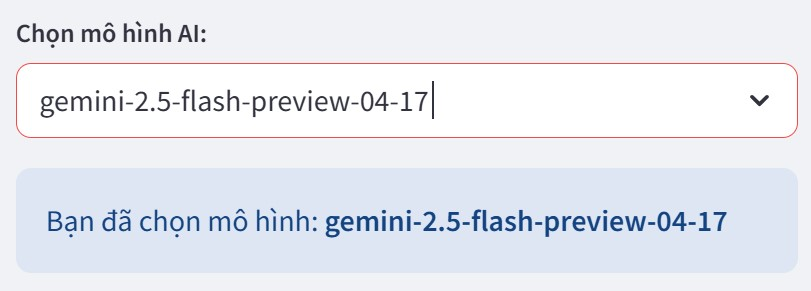
\includegraphics[width=0.55\linewidth]{img/21127739/research/research_choose_model.jpg}}
        \caption{Giao diện sidebar chọn mô hình của công cụ hỗ trợ nghiên cứu chủ đề}
        \label{fig:research_choose_model}
    \end{figure}
    \vspace*{-18pt}

    \item \textbf{Khu vực tùy chỉnh prompt:} Sử dụng \texttt{st.expander} để tạo một khu vực có thể mở rộng/thu gọn (xem Hình~\ref{fig:research_prompt_area}), chứa:
    \begin{itemize}
        \item Một vùng nhập văn bản lớn (\texttt{st.text\_area}) hiển thị prompt hiện tại (mặc định hoặc đã tùy chỉnh) và cho phép người dùng chỉnh sửa.

        \item Hai nút bấm (\texttt{st.button}) được đặt trong hai cột (\texttt{st.columns}): "\textbf{Cập nhật prompt}" để lưu thay đổi và "\textbf{Khôi phục prompt mặc định}" để quay lại nội dung gốc từ file \texttt{user\_prompt\_template.md}.
        
        \item Thông báo thành công (\texttt{st.success}) được hiển thị khi cập nhật hoặc khôi phục prompt.  
    \end{itemize}
    \vspace*{-10pt}
    % Insert image
    \begin{figure}[H]
        \centering
        % Insert border box
        \frame{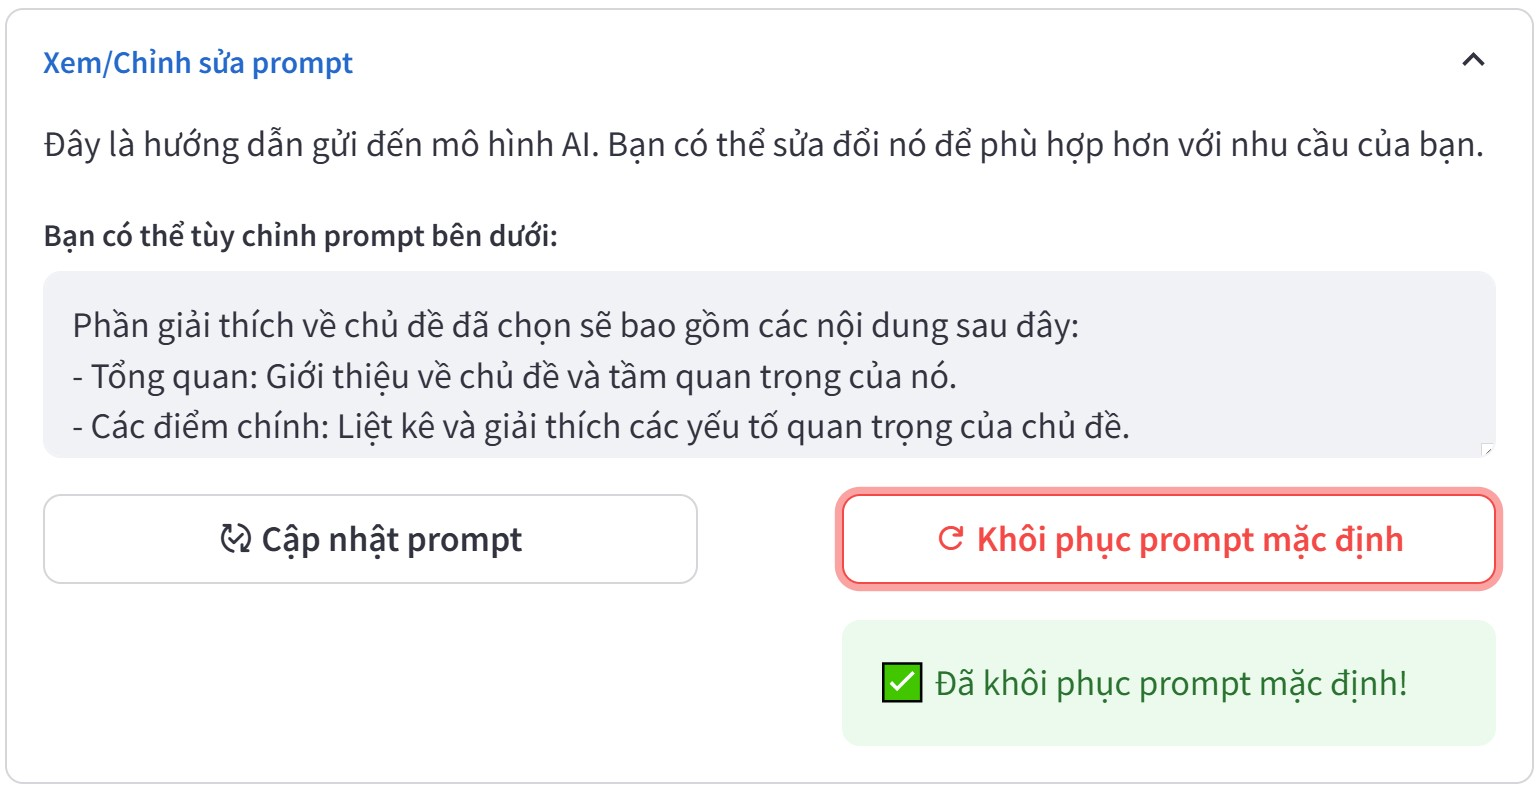
\includegraphics[width=0.8\linewidth]{img/21127739/research/research_prompt_area.jpg}}
        \caption{Giao diện khu vực tùy chỉnh prompt của công cụ hỗ trợ nghiên cứu chủ đề}
        \label{fig:research_prompt_area}
    \end{figure}
    \vspace*{-16pt}

    \item \textbf{Khu vực nhập chủ đề:} Một vùng nhập văn bản (\texttt{st.text\_area}) để người dùng nhập chủ đề cần nghiên cứu. Có một ví dụ minh họa (\texttt{st.expander}) để hướng dẫn người dùng ngay bên dưới (xem Hình~\ref{fig:research_topic_area}).
    
    \item \textbf{Nút tạo kết quả:} Nút "\textbf{Tiến hành nghiên cứu}" (\texttt{st.button} với \texttt{type="primary"}) để tiến hành gửi yêu cầu đến API (xem Hình~\ref{fig:research_topic_area}). Hệ thống sẽ kiểm tra xem người dùng đã nhập chủ đề hay chưa, nếu chưa sẽ hiển thị thông báo yêu cầu nhập chủ đề (\texttt{st.warning}).
    \vspace*{-4pt}
    % Insert image
    \begin{figure}[H]
        \centering
        % Insert border box
        \frame{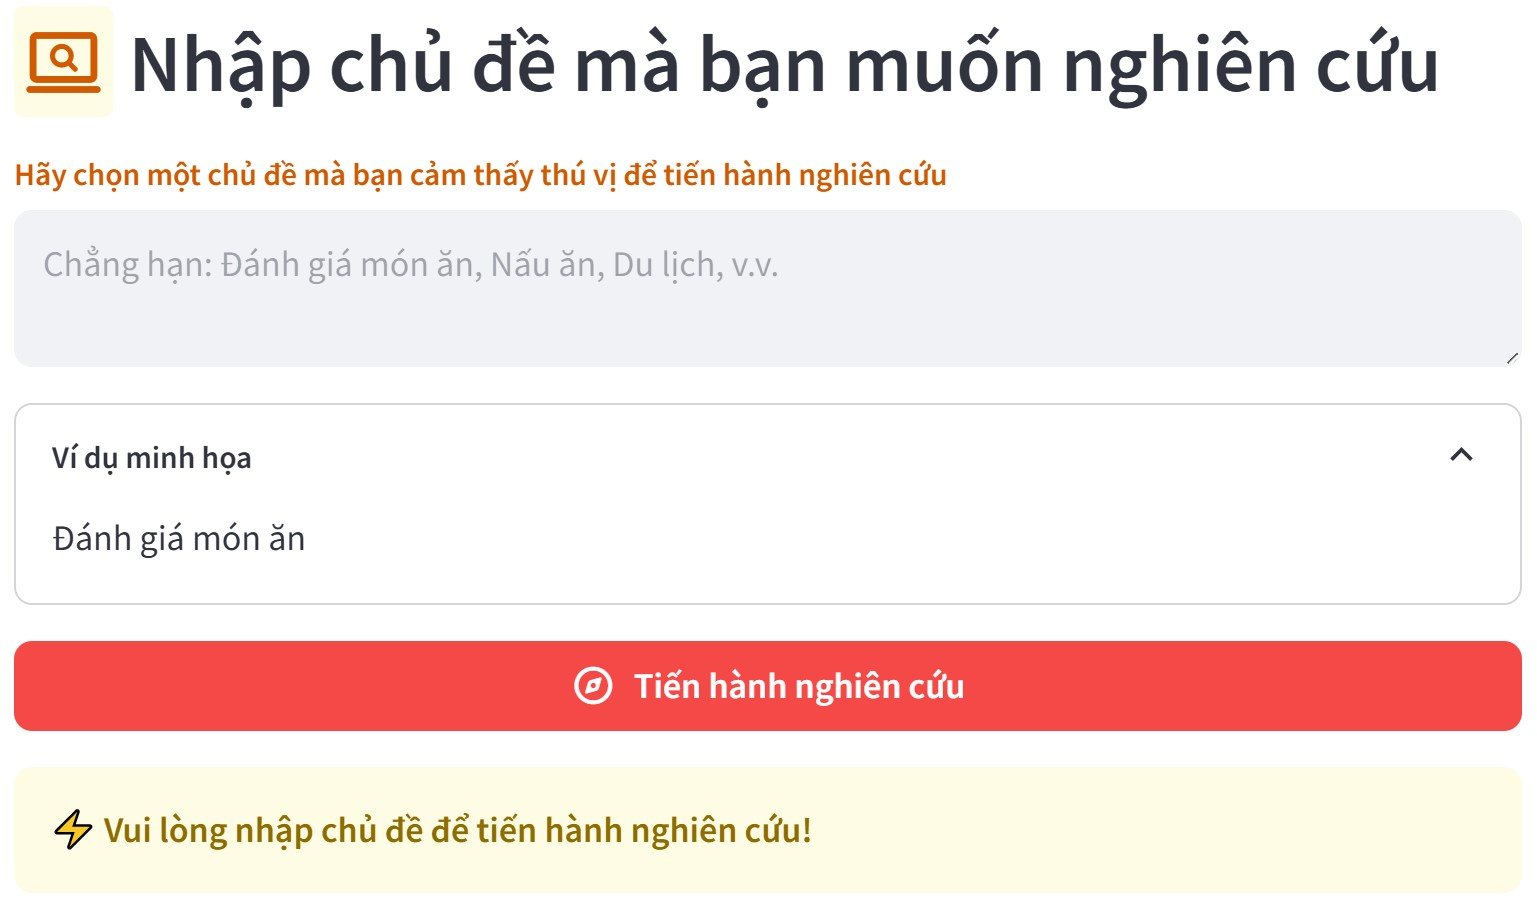
\includegraphics[width=0.8\linewidth]{img/21127739/research/research_topic_area.jpg}}
        \caption{Giao diện khu vực nhập chủ đề của công cụ hỗ trợ nghiên cứu chủ đề}
        \label{fig:research_topic_area}
    \end{figure}
    
    \item \textbf{Hiển thị kết quả:} Kết quả trả về từ API (sau khi chuẩn hóa) được hiển thị dưới dạng Markdown (\texttt{st.markdown}) trong khu vực chính (xem Hình~\ref{fig:research_result_area}). Khu vực này có thể cuộn để xem toàn bộ nội dung. Nội dung được phân chia thành các phần rõ ràng theo cấu trúc đã định nghĩa trong prompt, giúp người dùng dễ dàng theo dõi và hiểu thông tin.
    % Insert image
    \begin{figure}[H]
        \centering
        % Insert border box
        \frame{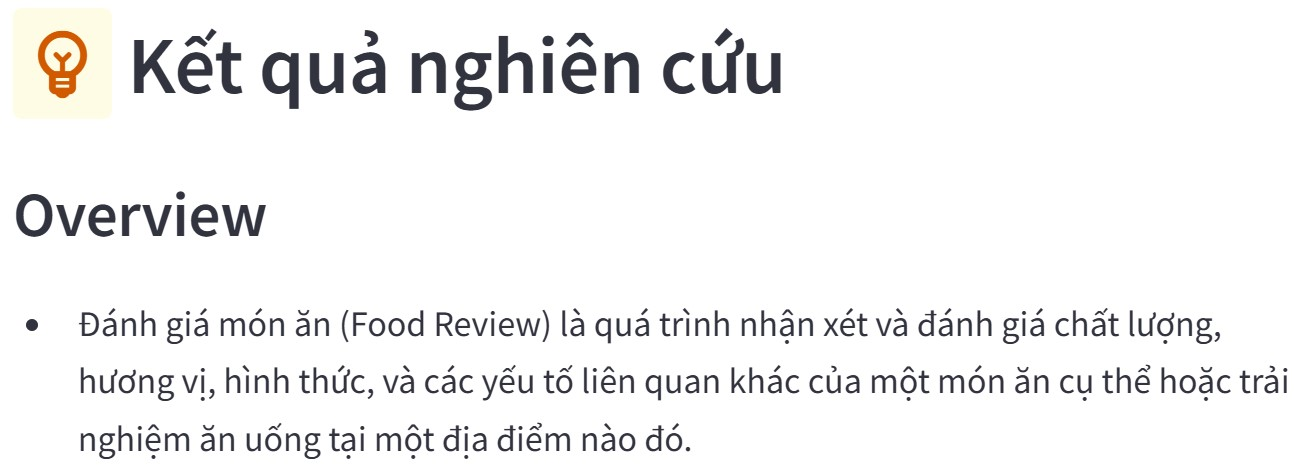
\includegraphics[width=0.67\linewidth]{img/21127739/research/research_result_area.jpg}}
        \caption{Giao diện khu vực hiển thị kết quả của công cụ hỗ trợ nghiên cứu chủ đề}
        \label{fig:research_result_area}
    \end{figure}
    \vspace*{-14pt}

    \item \textbf{Lưu kết quả:} Hai nút bấm (\texttt{st.button} và \texttt{st.download\_button}) được đặt trong hai cột (\texttt{st.columns}) dưới phần kết quả (xem Hình~\ref{fig:research_save_result}), cho phép người dùng:
    \begin{itemize}
        \item Sao chép kết quả vào clipboard (sử dụng thư viện \texttt{pyperclip}).

        \item Tải kết quả xuống dưới dạng file Markdown (\texttt{.md}).        
    \end{itemize}
    \vspace*{-4pt}
    % Insert image
    \begin{figure}[H]
        \centering
        % Insert border box
        \frame{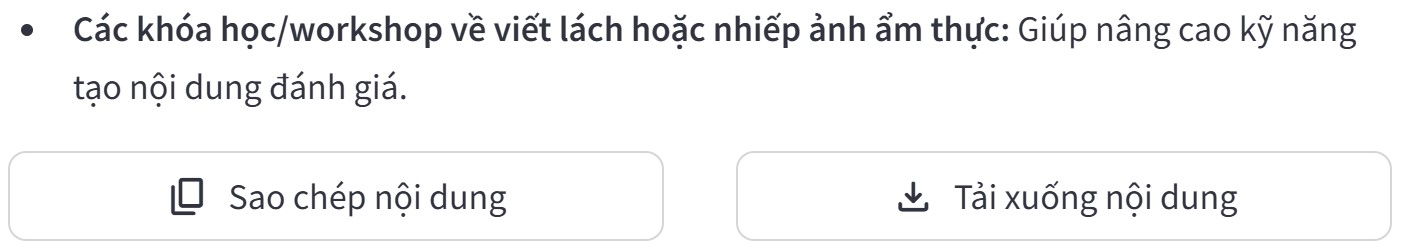
\includegraphics[width=0.67\linewidth]{img/21127739/research/research_save_result.jpg}}
        \caption{Giao diện khu vực lưu kết quả của công cụ hỗ trợ nghiên cứu chủ đề}
        \label{fig:research_save_result}
    \end{figure}
\end{enumerate}

\paragraph{Luồng tương tác của người dùng:} Người dùng sẽ thực hiện các bước sau để sử dụng công cụ:
\begin{enumerate}
    \item (Tùy chọn) Chọn mô hình AI từ sidebar.

    \item (Tùy chọn) Mở rộng khu vực prompt, xem và chỉnh sửa nếu cần, sau đó nhấn "Cập nhật prompt" hoặc "Khôi phục prompt mặc định".
    
    \item Nhập chủ đề muốn nghiên cứu vào ô văn bản.
    
    \item Nhấn nút "Tiến hành nghiên cứu".
    
    \item Chờ đợi trong khi hệ thống hiển thị trạng thái "Đang nghiên cứu..." (\texttt{st.spinner}).
    
    \item Xem kết quả được hiển thị.
    
    \item (Tùy chọn) Sao chép hoặc tải xuống kết quả.
\end{enumerate}

\subsubsection{Kỹ thuật Prompting}

Hiệu quả của công cụ phụ thuộc rất lớn vào cách thiết kế prompt để giao tiếp với mô hình Gemini. Nhóm đã áp dụng phương pháp sử dụng kết hợp \textbf{System Prompt} và \textbf{User Prompt} để tối ưu hóa khả năng tạo nội dung của mô hình:
\begin{enumerate}
    \item \textbf{System Prompt (\texttt{system\_prompt\_template.md}):}
    \begin{itemize}
        \item \textbf{Mục đích:} Định nghĩa vai trò và hướng dẫn tổng quát cho mô hình AI. Prompt này yêu cầu mô hình đóng vai là ``\textit{chuyên gia nghiên cứu với kiến thức sâu rộng}''.

        \item \textbf{Định dạng đầu ra:} Quan trọng nhất, system prompt yêu cầu mô hình trả lời theo định dạng Markdown với một cấu trúc gồm 7 phần rõ ràng: \texttt{Overview}, \texttt{Key Points}, \texttt{Examples}, \texttt{Challenges}, \texttt{Best Practices}, \texttt{Trends}, và \texttt{Resources}. Nó cũng nhấn mạnh các yêu cầu về tính rõ ràng, súc tích, chính xác và việc chỉ trả về nội dung bên trong khối Markdown.
        
        \item \textbf{Kỹ thuật:} Sử dụng kỹ thuật "\textbf{Role Playing}" (đóng vai) và "\textbf{Output Formatting}" (định dạng đầu ra) để kiểm soát hành vi và cấu trúc kết quả của LLM.
    \end{itemize}

    \item \textbf{User Prompt (\texttt{user\_prompt\_template.md} và tùy chỉnh của người dùng):}
    \begin{itemize}
        \item \textbf{Mục đích:} Cung cấp yêu cầu cụ thể hơn về nội dung cho từng phần trong cấu trúc đã định nghĩa ở system prompt. Prompt mặc định liệt kê lại các phần mong muốn và mô tả ngắn gọn nội dung của từng phần.

        \item \textbf{Tính linh hoạt:} Người dùng có thể tùy chỉnh user prompt này thông qua giao diện (\texttt{st.text\_area}). Ví dụ, họ có thể yêu cầu tập trung sâu hơn vào phần "Challenges" hoặc bổ sung một phần mới như "Target Audience".
        
        \item \textbf{Kết hợp:} Khi gửi yêu cầu đến API, system prompt được gửi trước, theo sau là một câu dẫn (``\textit{Hãy giúp tôi tạo ra một bài giải thích chi tiết về chủ đề [topic].}'') và cuối cùng là nội dung user prompt (mặc định hoặc đã tùy chỉnh).
    \end{itemize}

    \item \textbf{Khôi phục Prompt:} Chức năng khôi phục về prompt mặc định (\texttt{default\_user\_prompt}) đảm bảo người dùng luôn có thể quay lại trạng thái ban đầu nếu việc tùy chỉnh không như ý.
\end{enumerate}

Kỹ thuật prompting này giúp đảm bảo tính nhất quán trong cấu trúc đầu ra, đồng thời mang lại sự linh hoạt cho người dùng để điều chỉnh nội dung theo nhu cầu nghiên cứu cụ thể.

\subsubsection{Tương tác với Gemini API và Xử lý kết quả}
\begin{enumerate}
    \item \textbf{Lựa chọn mô hình:} Như đã đề cập, người dùng có thể chọn các mô hình Gemini khác nhau. Hàm \texttt{read\_available\_gemini\_models} đọc danh sách các mô hình có sẵn từ file \texttt{models/gemini\_models.txt} và hiển thị trong \texttt{st.selectbox}. Việc chọn mô hình nhanh hơn (\texttt{gemini-2.0-flash}, \texttt{gemini-2.5-flash}) sẽ cho kết quả nhanh hơn nhưng có thể kém chi tiết hơn so với mô hình mạnh hơn (\texttt{gemini-2.5-pro}).
    
    \item \textbf{Gửi yêu cầu:} Khi người dùng nhấn nút "Tiến hành nghiên cứu", hàm \texttt{generate\_content} (trong file \texttt{research.py}, gọi đến \texttt{client.models.generate\_content} của thư viện \texttt{google-\\genai}) được thực thi. Hàm này nhận vào system prompt, user prompt (đã được định dạng cùng với chủ đề) và tên mô hình đã chọn. API key được sử dụng để xác thực yêu cầu. (\textit{Quá trình này thường mất khoảng 15 giây.})
    
    \item \textbf{Nhận và Chuẩn hóa phản hồi:} Gemini API trả về một đối tượng response. Phần nội dung văn bản (\texttt{response.text}) thường được bao bọc trong khối mã Markdown (nội dung chính được bao bọc bởi các ký tự đánh dấu). Hàm \texttt{standardize\_response} được sử dụng để loại bỏ các ký tự đánh dấu không cần thiết, chỉ giữ lại nội dung Markdown thuần túy.
    
    \item \textbf{Hiển thị và Lưu trữ:} Kết quả Markdown đã chuẩn hóa được hiển thị trực tiếp trên giao diện bằng \texttt{st.markdown}. Đồng thời, kết quả này được lưu vào \texttt{st.session\_state.last\_re-\\search\_response} để có thể sử dụng cho chức năng sao chép và tải xuống.
    
    \item \textbf{Sao chép và Tải xuống:}
    \begin{itemize}
        \item Nút "Sao chép nội dung" sử dụng thư viện \texttt{pyperclip} (\texttt{pyperclip.copy()}) để đưa nội dung trong \texttt{st.session\_state.last\_research\_response} vào clipboard hệ thống (\textit{tiện lợi cho việc dán vào tài liệu hoặc ứng dụng khác}).
        
        \item Nút "Tải xuống nội dung" sử dụng \texttt{st.download\_button}, truyền vào nội dung (có thể thêm tiêu đề ``\texttt{\# Chủ đề: [topic]}'') và định dạng file là \texttt{research\_topic.md} với kiểu MIME là \texttt{text/plain} (\textit{phù hợp cho chỉnh sửa hoặc lưu trữ lâu dài}).
    \end{itemize}
    
\end{enumerate}

\subsubsection{Minh họa cách sử dụng công cụ}

% Providing a practical example
Để minh họa cách công cụ hoạt động, nhóm đã quay video hướng dẫn sử dụng công cụ này, người dùng có thể tham khảo video demo tại \href{https://youtu.be/m-cdmfVc2rk?list=PL3SfxVDJ_Zc6DvBKVd6xUc-exmt0AyA7x&t=246}{đây} (\textit{từ phút 4:10 đến 8:32}). Trong ví dụ minh họa, người dùng muốn nghiên cứu về chủ đề "Đánh giá món ăn" (Food Review) để tạo video TikTok. Ví dụ này cho thấy công cụ giúp người dùng nhanh chóng thu thập thông tin có cấu trúc, hỗ trợ quá trình sáng tạo nội dung.

\subsection{Công cụ gợi ý cách quay video ẩm thực}

% Insert image
\begin{figure}[H]
    \centering
    % Insert border box
    \frame{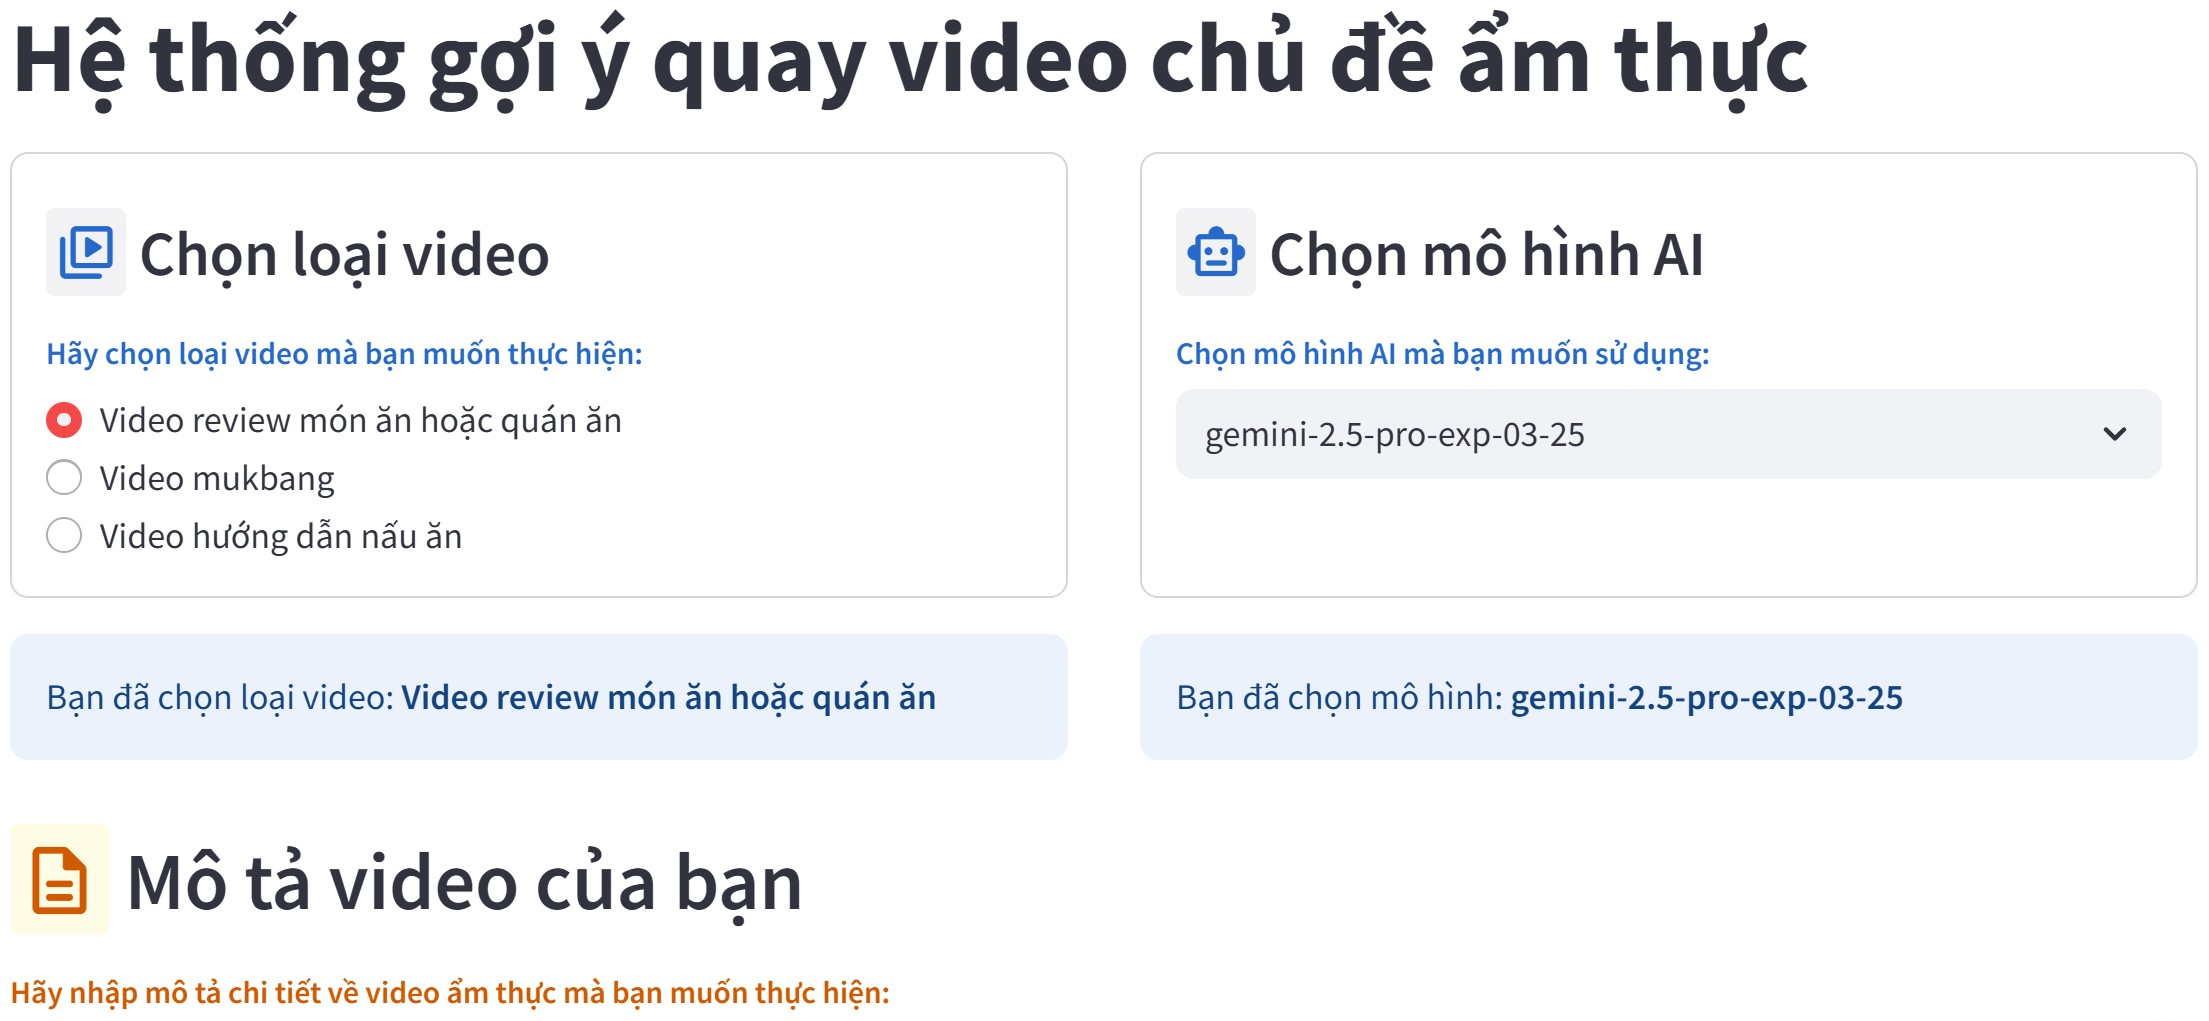
\includegraphics[width=0.99\linewidth]{img/21127739/suggestion/suggestion_main_page.jpg}}
    \caption{Giao diện chính của công cụ gợi ý cách quay video ẩm thực}
    \label{fig:suggestion_main_page}
\end{figure}

\subsubsection{Tổng quan}

Trong quy trình sáng tạo nội dung trên TikTok, sau giai đoạn lên ý tưởng và viết kịch bản, việc thực hiện các cảnh quay (filming) đóng vai trò then chốt, quyết định phần lớn chất lượng hình ảnh và cảm xúc của video thành phẩm. Đối với lĩnh vực ẩm thực, việc quay phim đòi hỏi sự chú ý đặc biệt đến các yếu tố như góc máy làm nổi bật món ăn, ánh sáng hấp dẫn, âm thanh sống động và cách thể hiện tương tác tự nhiên. Tuy nhiên, không phải nhà sáng tạo nội dung nào cũng có đủ kinh nghiệm hoặc kiến thức chuyên sâu về kỹ thuật quay phim cho từng thể loại video ẩm thực cụ thể.

Để giải quyết thách thức này và bổ sung vào bộ công cụ hỗ trợ phát triển kênh TikTok, nhóm đã xây dựng \textbf{Công cụ Gợi ý Cách quay Video Ẩm thực}. Công cụ này hoạt động như một \textbf{cố vấn sản xuất ảo}, cung cấp những lời khuyên và gợi ý kỹ thuật quay phim chi tiết, được cá nhân hóa dựa trên ý tưởng video và thể loại ẩm thực mà người dùng lựa chọn. Tương tự công cụ nghiên cứu chủ đề, công cụ này cũng khai thác sức mạnh của Mô hình Ngôn ngữ Lớn (LLM) tiên tiến thông qua \href{https://ai.google.dev/}{Gemini API}, tập trung vào kỹ thuật prompting để tạo ra các gợi ý chuyên sâu. Phần này sẽ đi sâu vào phân tích mục tiêu, kiến trúc, các kỹ thuật chính và quy trình hoạt động của công cụ gợi ý quay video.

\subsubsection{Mục tiêu và Lợi ích}

\noindent
Công cụ được xây dựng với các mục tiêu cụ thể sau:
\begin{enumerate}
    \item \textbf{Nâng cao chất lượng hình ảnh:} Cung cấp các gợi ý về góc quay, ánh sáng, bố cục để giúp video trông chuyên nghiệp và hấp dẫn hơn về mặt thị giác.

    \item \textbf{Tối ưu hóa kỹ thuật quay:} Đề xuất các kỹ thuật quay phù hợp (slow-motion, cận cảnh, góc nhìn thứ nhất, v.v.) cho từng thể loại và nội dung cụ thể.
    
    \item \textbf{Cải thiện âm thanh:} Gợi ý cách thu âm, xử lý tạp âm và lựa chọn nhạc nền phù hợp để tăng trải nghiệm nghe của khán giả.
    
    \item \textbf{Tăng tính hấp dẫn của nội dung:} Đưa ra lời khuyên về cách tương tác, kể chuyện và trình bày món ăn một cách lôi cuốn.
    
    \item \textbf{Hỗ trợ theo thể loại:} Cung cấp gợi ý chuyên biệt cho các thể loại video ẩm thực phổ biến (review, nấu ăn, mukbang).
    
    \item \textbf{Tiết kiệm thời gian chuẩn bị:} Giúp người dùng, đặc biệt là những người mới, có sự chuẩn bị tốt hơn cho buổi quay, giảm thiểu thời gian thử nghiệm và sai sót.
\end{enumerate}

\subsubsection{Kiến trúc và Công nghệ sử dụng}

\noindent
Công cụ gợi ý quay video được triển khai dưới dạng ứng dụng web, sử dụng các thành phần công nghệ tương tự như công cụ nghiên cứu chủ đề:
\begin{enumerate}
    \item \textbf{Framework ứng dụng web:} \textbf{Streamlit} tiếp tục được sử dụng để xây dựng giao diện người dùng thân thiện và các thành phần tương tác (tham khảo file \texttt{suggestion.py}).

    \item \textbf{Mô hình Ngôn ngữ Lớn (LLM):} Công cụ dựa vào khả năng hiểu ngữ cảnh, kiến thức chuyên môn (được mô phỏng qua prompt) và khả năng tạo văn bản của các mô hình \textbf{Gemini API} để đưa ra các gợi ý quay phim.
    
    \item \textbf{Thư viện tương tác với API:} Thư viện \texttt{google-genai} được dùng để giao tiếp với Gemini API.
    
    \item \textbf{Kỹ thuật Prompting theo ngữ cảnh:} Điểm nhấn kỹ thuật của công cụ này là việc sử dụng các \textbf{prompt chuyên biệt} cho từng thể loại video ẩm thực, kết hợp với mô tả ý tưởng của người dùng để tạo ra gợi ý phù hợp nhất.
    
    \item \textbf{Quản lý trạng thái:} \textbf{Streamlit Session State} (\texttt{st.session\_state}) được dùng để lưu trữ gợi ý gần nhất được tạo ra, cho phép người dùng xem lại và thực hiện các thao tác lưu trữ.
    
    \item \textbf{Caching:} Kỹ thuật caching (\texttt{@st.cache\_data}) được áp dụng cho việc đọc danh sách mô hình và nội dung các file prompt template, tối ưu hóa hiệu năng ứng dụng.
\end{enumerate}

\subsubsection{Thiết kế giao diện người dùng và Luồng tương tác}

\paragraph{Giao diện người dùng:} Giao diện người dùng được thiết kế để người dùng dễ dàng nhập thông tin và nhận gợi ý:
\begin{enumerate}
    \item \textbf{Chọn loại video và mô hình AI:} (Xem Hình~\ref{fig:suggestion_choose_video_type_and_model})
    \begin{itemize}
        \item Sử dụng hai cột (\texttt{st.columns}) để bố trí các lựa chọn.

        \item \textbf{Chọn loại video:} Người dùng chọn một trong ba loại video ẩm thực (\textit{Video review món ăn hoặc quán ăn}, \textit{Video mukbang}, \textit{Video hướng dẫn nấu ăn}) thông qua nút \texttt{st.radio}. Danh sách các loại video được định nghĩa trong biến \texttt{VIDEO\_TYPES}.
        
        \item \textbf{Chọn mô hình AI:} Người dùng chọn mô hình Gemini mong muốn từ danh sách (đọc từ file \texttt{models/gemini\_models.txt}) bằng \texttt{st.selectbox}.
        
        \item Thông tin về lựa chọn của người dùng được hiển thị xác nhận bằng \texttt{st.info}.
    \end{itemize}
    % Insert image
    \begin{figure}[H]
        \centering
        % Insert border box
        \frame{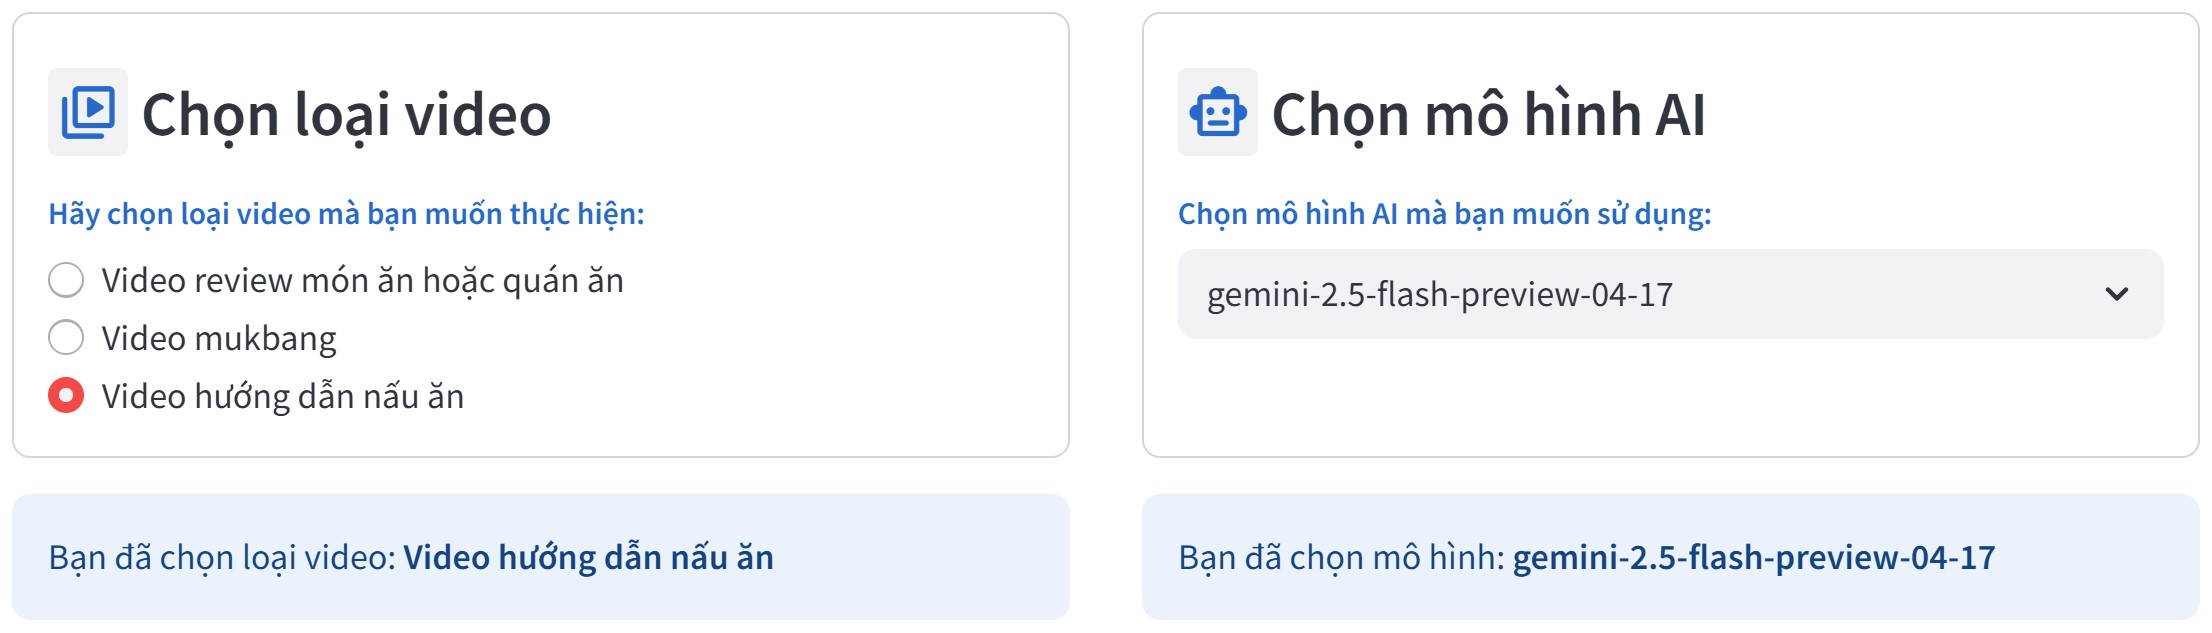
\includegraphics[width=0.9\linewidth]{img/21127739/suggestion/suggestion_choose_video_type_and_model.jpg}}
        \caption{Giao diện chọn loại video và mô hình AI của công cụ gợi ý cách quay video ẩm thực}
        \label{fig:suggestion_choose_video_type_and_model}
    \end{figure}

    \item \textbf{Nhập mô tả video:} (Xem Hình~\ref{fig:suggestion_input_description})
    \begin{itemize}
        \item Một vùng nhập văn bản lớn (\texttt{st.text\_area}) cho phép người dùng mô tả chi tiết ý tưởng video của họ (món ăn, địa điểm, phong cách, mục tiêu, v.v.).

        \item Có một ví dụ minh họa (\texttt{st.expander}) để người dùng tham khảo cách mô tả hiệu quả.
    \end{itemize}
    \item \textbf{Nút tạo gợi ý:} Nút "Tạo gợi ý" (\texttt{st.button} với \texttt{type="primary"}) để bắt đầu quá trình tạo gợi ý. Hệ thống sẽ kiểm tra xem người dùng đã nhập mô tả hay chưa, nếu chưa sẽ hiển thị thông báo yêu cầu nhập mô tả thông qua \texttt{st.warning} (xem Hình~\ref{fig:suggestion_input_description}).
    % Insert image
    \begin{figure}[H]
        \centering
        % Insert border box
        \frame{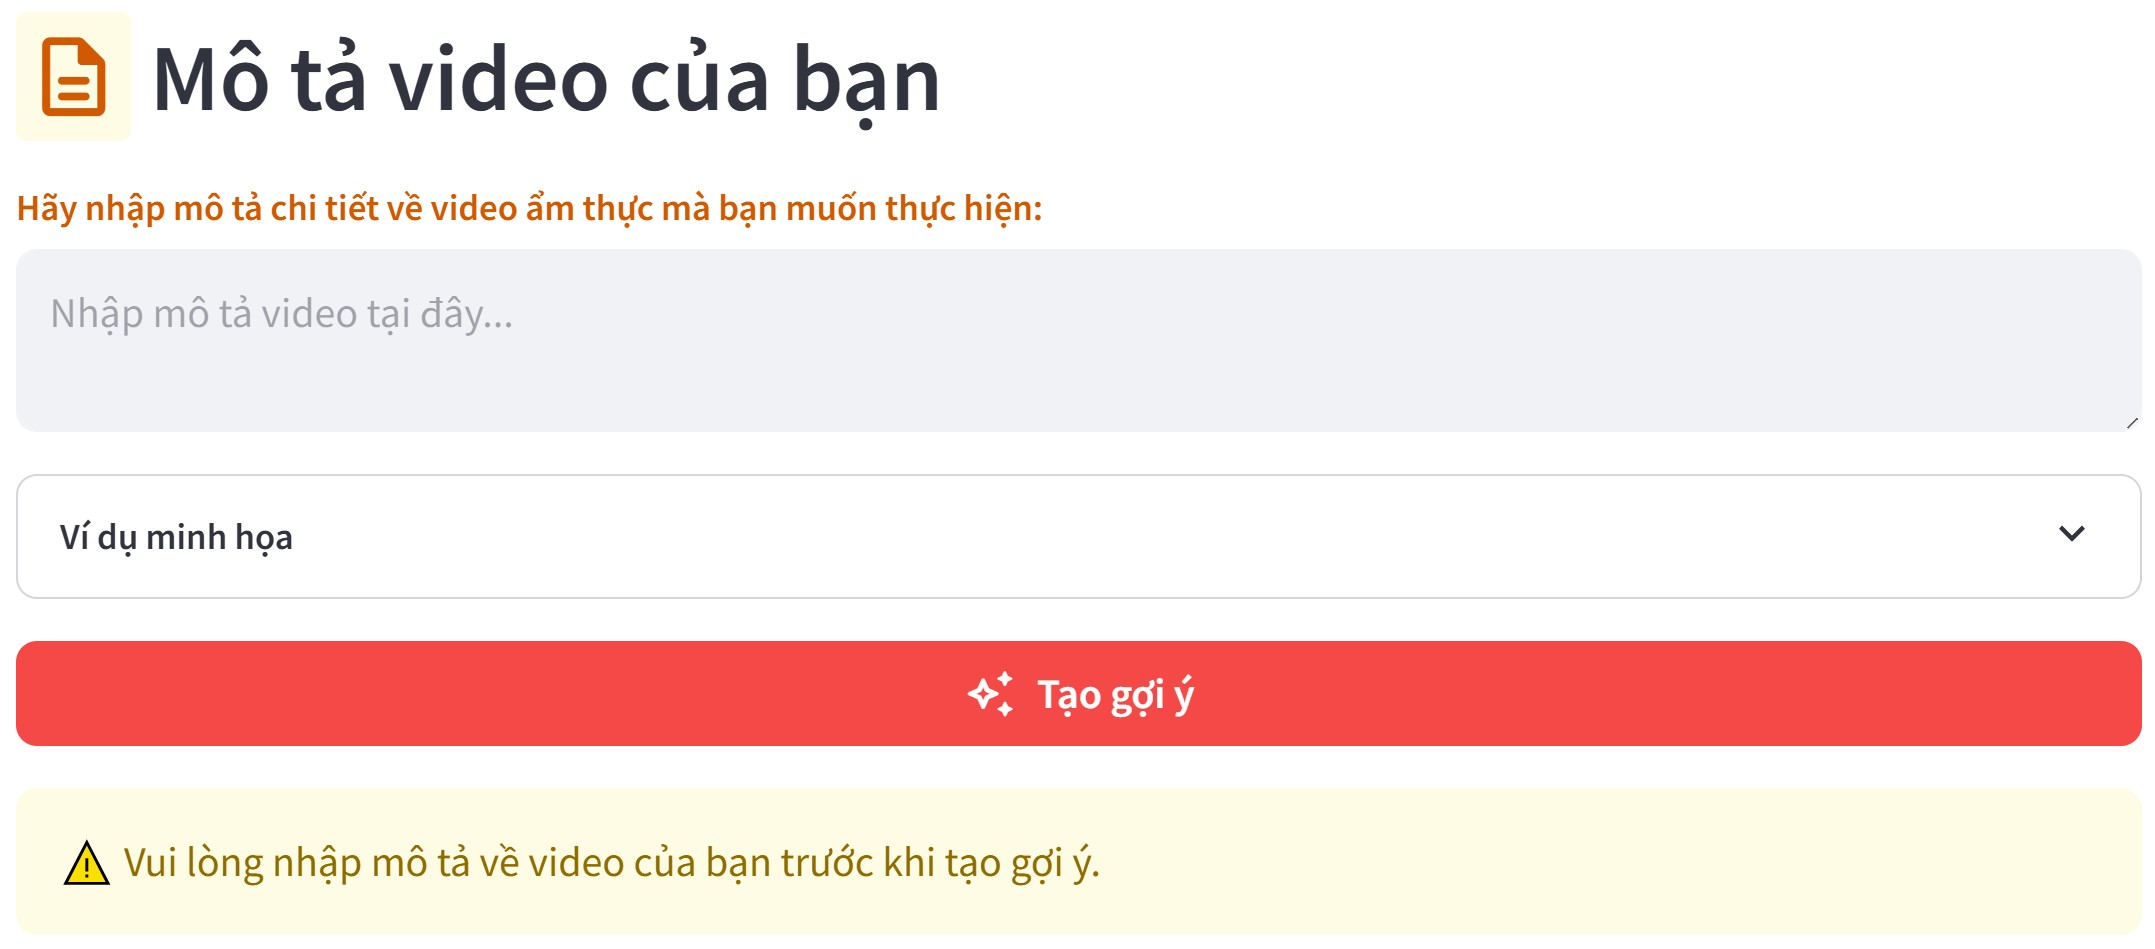
\includegraphics[width=0.9\linewidth]{img/21127739/suggestion/suggestion_input_description.jpg}}
        \caption{Giao diện nhập mô tả video của công cụ gợi ý cách quay video ẩm thực}
        \label{fig:suggestion_input_description}
    \end{figure}

    \item \textbf{Hiển thị gợi ý:} (Xem Hình~\ref{fig:suggestion_result})
    \begin{itemize}
        \item Trong khi chờ đợi, \texttt{st.spinner} hiển thị thông báo "Đang tạo gợi ý...".

        \item Kết quả gợi ý (dạng Markdown) trả về từ API được lưu vào \texttt{st.session\_state.sug-\\gestion} và hiển thị trên giao diện bằng \texttt{st.markdown}.
    \end{itemize}
    % Insert image
    \begin{figure}[H]
        \centering
        % Insert border box
        \frame{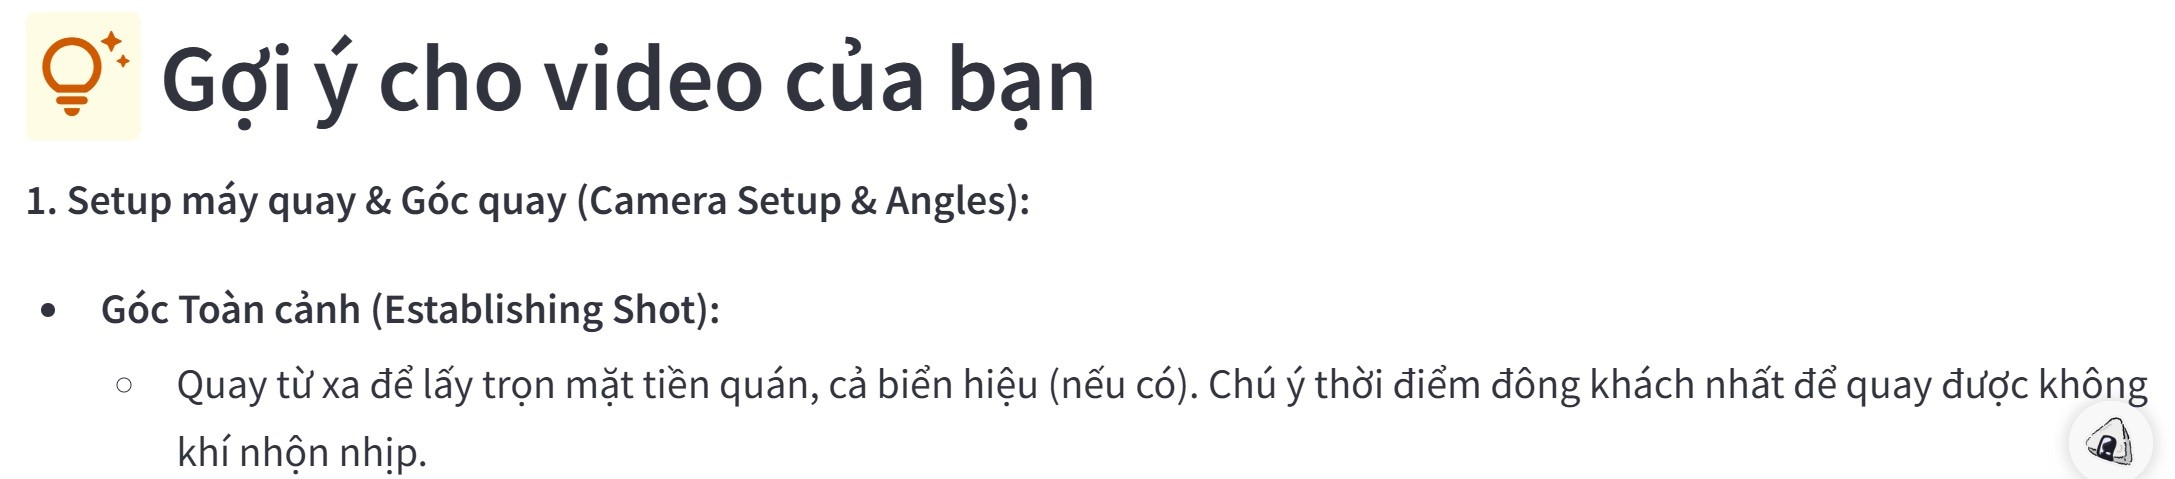
\includegraphics[width=0.9\linewidth]{img/21127739/suggestion/suggestion_result.jpg}}
        \caption{Giao diện hiển thị gợi ý của công cụ gợi ý cách quay video ẩm thực}
        \label{fig:suggestion_result}
    \end{figure}

    \item \textbf{Lưu kết quả:} (Xem Hình~\ref{fig:suggestion_save_result}) Tương tự công cụ nghiên cứu, hai nút bấm trong hai cột (\texttt{st.columns}) cho phép:
    \begin{itemize}
        \item Sao chép gợi ý vào clipboard (\texttt{pyperclip.copy()}).
        
        \item Tải gợi ý xuống dưới dạng file Markdown (\texttt{.md}) bằng \texttt{st.download\_button}.
    \end{itemize}
    % Insert image
    \begin{figure}[H]
        \centering
        % Insert border box
        \frame{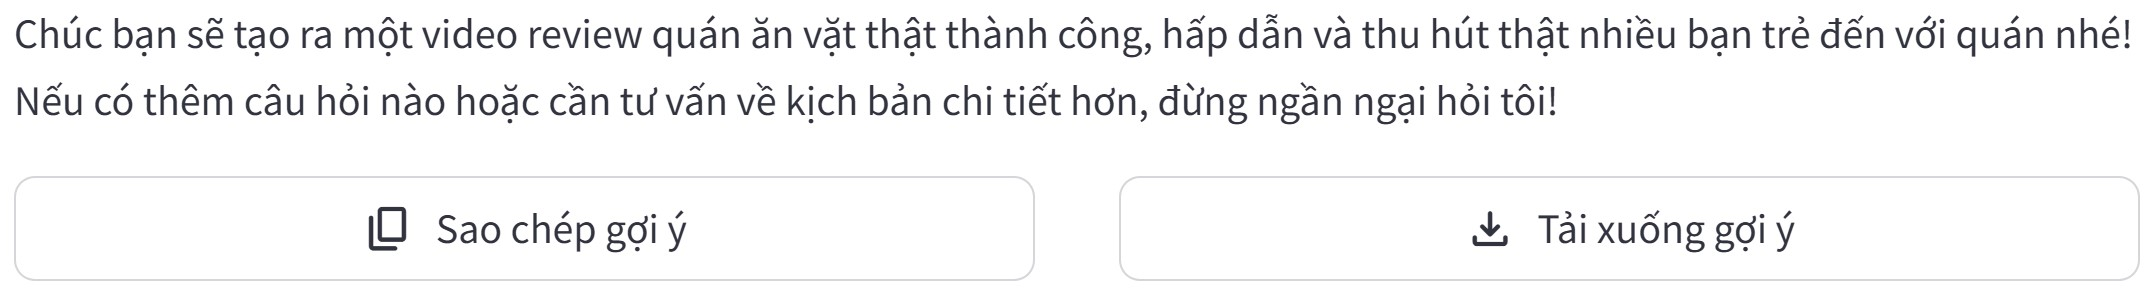
\includegraphics[width=0.9\linewidth]{img/21127739/suggestion/suggestion_save_result.jpg}}
        \caption{Giao diện lưu kết quả của công cụ gợi ý cách quay video ẩm thực}
        \label{fig:suggestion_save_result}
    \end{figure}

\end{enumerate}

\paragraph{Luồng tương tác của người dùng:} Người dùng sẽ thực hiện các bước sau để sử dụng công cụ:
\begin{enumerate}
    \item Chọn loại video ẩm thực muốn thực hiện.

    \item (Tùy chọn) Chọn mô hình AI muốn sử dụng.
    
    \item Nhập mô tả chi tiết về ý tưởng video.
    
    \item Nhấn nút "Tạo gợi ý".
    
    \item Xem các gợi ý chi tiết được hiển thị.
    
    \item (Tùy chọn) Sao chép hoặc tải xuống các gợi ý.
\end{enumerate}

\subsubsection{Kỹ thuật Prompting chuyên biệt theo thể loại video}

Đây là yếu tố kỹ thuật cốt lõi giúp công cụ đưa ra những gợi ý phù hợp và chuyên sâu. Thay vì dùng một prompt chung, công cụ sử dụng các prompt riêng biệt được thiết kế cho từng thể loại video ẩm thực:
\begin{enumerate}
    \item \textbf{Cấu trúc Prompt:} Mỗi prompt template (lưu trong các file \texttt{.md} tương ứng: \texttt{food\_review-\\\_template.md}, \texttt{cooking\_template.md}, \texttt{mukbang\_template.md}) đều có cấu trúc chung:
    \begin{itemize}
        \item \textbf{Định nghĩa vai trò (Role Playing):} Yêu cầu LLM đóng vai là "chuyên gia sản xuất video chuyên nghiệp" với kinh nghiệm trong thể loại video tương ứng (review, nấu ăn, hoặc mukbang).

        \item \textbf{Xác định đầu vào:} Nêu rõ rằng người dùng sẽ cung cấp thông tin/mô tả về video họ muốn làm.
        
        \item \textbf{Yêu cầu đầu ra:} Liệt kê chi tiết các hạng mục cần gợi ý, được trình bày dưới dạng danh sách gạch đầu dòng với các tiêu đề in đậm (định dạng Markdown). Các hạng mục này bao gồm những khía cạnh quan trọng nhất của việc quay phim ẩm thực:
        \begin{itemize}
            \item \textit{Setup máy quay \& Góc quay}

            \item \textit{Ánh sáng \& Âm thanh}
            
            \item \textit{Giải thích \& Hướng dẫn chi tiết} (cho video nấu ăn) hoặc \textit{Chi tiết về phỏng vấn \& giao tiếp} (cho video review) hoặc \textit{Nêu cảm nhận \& Tương tác với khán giả} (cho video mukbang)
            
            \item \textit{Hiệu ứng \& Chuyển cảnh}
            
            \item \textit{Storytelling \& CTA}
            
            \item \textit{SEO \& Thương hiệu} (cho video review)
        \end{itemize}

        \item \textbf{Yêu cầu định dạng:} Yêu cầu trả lời bằng định dạng Markdown.
    \end{itemize}

    \item \textbf{Nội dung chuyên biệt:} Mặc dù có cấu trúc chung, nội dung yêu cầu chi tiết trong từng hạng mục của mỗi prompt được điều chỉnh để phù hợp với đặc thù của thể loại đó:
    \begin{itemize}
        \item \textbf{Review:} Nhấn mạnh vào góc quay đa dạng (toàn cảnh quán, cận cảnh món ăn), cách phỏng vấn chủ quán, xây dựng câu chuyện, tạo không khí đặc trưng của quán.
        
        \item \textbf{Nấu ăn:} Tập trung vào góc quay chi tiết các bước chế biến, ánh sáng làm nổi bật món ăn, giải thích rõ ràng, tạo không khí ấm cúng trong bếp.
        
        \item \textbf{Mukbang:} Chú trọng góc quay thể hiện cảm xúc khi ăn, âm thanh ASMR (nếu có), cách tương tác tự nhiên, tạo không khí vui vẻ, thân mật.
    \end{itemize}
    
    \item \textbf{Kết hợp prompt và mô tả từ người dùng:} Khi người dùng chọn loại video và nhập mô tả, hàm \texttt{generate\_suggestion} (trong file \texttt{suggestion.py}) sẽ:
    \begin{itemize}
        \item Xác định file prompt template tương ứng dựa trên \texttt{video\_type} (thông qua dictionary \texttt{VIDEO\_TYPE\_TO\_PROMPT}).
        
        \item Đọc nội dung prompt từ file đó bằng hàm \texttt{read\_prompt\_file} (có sử dụng decorator \texttt{@st.cache\_data}).
        
        \item Gửi nội dung prompt này (đóng vai trò system prompt/hướng dẫn) cùng với \texttt{user\_des-\\cription} (mô tả của người dùng) đến Gemini API.
    \end{itemize}
\end{enumerate}

Cách tiếp cận này cho phép LLM hiểu rõ ngữ cảnh (thể loại video) và yêu cầu cụ thể (mô tả của người dùng), từ đó đưa ra những gợi ý quay phim mang tính chuyên môn và sát với thực tế hơn.

\subsubsection{Tương tác với Gemini API và Xử lý kết quả}

\noindent
Quy trình tương tác với API và xử lý kết quả tương tự như công cụ nghiên cứu chủ đề:
\begin{enumerate}
    \item \textbf{Lựa chọn mô hình AI:} Người dùng chọn mô hình AI qua \texttt{st.selectbox}, mỗi mô hình có đặc điểm riêng về độ chi tiết và tốc độ phản hồi. Một số mô hình tiêu biểu bao gồm:
    \begin{itemize}
        \item \textbf{Gemini-2.5-pro}: Mô hình thử nghiệm tiên tiến nhất, được Google công bố vào tháng 3 năm 2025, cung cấp câu trả lời chi tiết nhưng có thể chậm hơn do tính chất thử nghiệm.
        
        \item \textbf{Gemini-2.0-flash}: Mô hình ổn định, được Google khuyến nghị cho các nhà phát triển, nổi bật với tốc độ phản hồi nhanh và chất lượng tốt trên nhiều tác vụ.
        
        \item \textbf{Gemini-2.5-flash}: Mô hình thử nghiệm mới, ra mắt vào giữa tháng 4 năm 2025, cân bằng giữa tốc độ của \textbf{Gemini-2.0-flash} và độ chi tiết của \textbf{Gemini-2.5-pro}.
    \end{itemize}

    \item \textbf{Gửi yêu cầu:} Hàm \texttt{generate\_suggestion} gọi \texttt{client.models.generate\_content} với prompt template phù hợp, mô tả của người dùng và tên mô hình đã chọn.
    
    \item \textbf{Nhận và Hiển thị phản hồi:} Kết quả dạng text được trả về và hiển thị bằng \texttt{st.markdown}.
    
    \item \textbf{Lưu trữ và Tương tác:} Kết quả được lưu vào \texttt{st.session\_state} để hỗ trợ sao chép (\texttt{pyperclip.copy}) và tải xuống (\texttt{st.download\_button} với tên file \texttt{video\_suggestion.md}).
\end{enumerate}

\subsubsection{Minh họa cách sử dụng công cụ}

% Providing a practical example
Để minh họa cách công cụ hoạt động, nhóm đã quay video hướng dẫn sử dụng công cụ này, người dùng có thể tham khảo video demo tại \href{https://youtu.be/m-cdmfVc2rk?list=PL3SfxVDJ_Zc6DvBKVd6xUc-exmt0AyA7x&t=512}{đây} (\textit{từ phút 8:32 đến 11:04}). Trong ví dụ minh họa, người dùng muốn quay video review một quán ăn vặt dành cho học sinh sinh viên. Công cụ gợi ý cách quay video sẽ giúp người dùng có được những gợi ý chi tiết về cách quay, ánh sáng, âm thanh và cách tương tác với chủ quán để tạo ra một video hấp dẫn và chất lượng.

